% Straight up stealing preamble from Eli Holmes 
%%%%%%%%%%%%%%%%%%%%%%%%%%%%%%%%%%%%%%START PREAMBLE THAT IS THE SAME FOR ALL EXAMPLES
\documentclass{article}

%Required: You must have these
\usepackage{Sweave}
\usepackage{graphicx}
\usepackage{tabularx}
\usepackage{hyperref}
\usepackage{natbib}
\usepackage{pdflscape}
\usepackage{array}
\usepackage{gensymb}
\usepackage{authblk}
\renewcommand{\baselinestretch}{1.8}
%\usepackage{lineno}
%\usepackage[backend=bibtex]{biblatex}
%Strongly recommended
 %put your figures in one place
 
%you'll want these for pretty captioning
\usepackage[small]{caption}

\setkeys{Gin}{width=0.8\textwidth} %make the figs 50 perc textwidth
\setlength{\captionmargin}{30pt}
\setlength{\abovecaptionskip}{0pt}
\setlength{\belowcaptionskip}{10pt}
% manual for caption http://www.dd.chalmers.se/latex/Docs/PDF/caption.pdf

%Optional: I like to muck with my margins and spacing in ways that LaTeX frowns on
%Here's how to do that
 \topmargin -2cm 
 \oddsidemargin -0.04cm 
 \evensidemargin -0.04cm % same as oddsidemargin but for left-hand pages
 \textwidth 16.59cm
 \textheight 22.94cm 
 %\pagestyle{empty} % Uncomment if don't want page numbers
 %\parskip 7.2pt  % sets spacing between paragraphs
 %\renewcommand{\baselinestretch}{1.5} 	% Uncomment for 1.5 spacing between lines
\parindent 0pt% sets leading space for paragraphs
\usepackage[doublespacing]{setspace}
%\doublespacing

%Optional: I like fancy headers
\usepackage{fancyhdr}
\pagestyle{fancy}
\fancyhead[LO]{Soil moisture and plant phenology}
\fancyhead[RO]{2018}

%%%%%%%%%%%%%%%%%%%%%%%%%%%%%%%%%%%%%%END PREAMBLE THAT IS THE SAME FOR ALL EXAMPLES

%Start of the document
\begin{document}

% \SweaveOpts{concordance=TRUE}
\bibliographystyle{/Users/aileneettinger/citations/Bibtex/styles/ecol_let.bst}

\title{Soil moisture interacts with temperature to affect plant phenology}
\begin{singlespace}

\author[1,2,a]{A.K. Ettinger}
\author[3,b]{J.S. Dukes}
\author[4,c]{M.R. Johnston}
\author[5,d]{C.R. Rollinson}
\author[1,4,6,e]{E.M. Wolkovich}

\affil[1]{Arnold Arboretum of Harvard University, Boston, Massachusetts 02131, USA}

\affil[2]{Tufts University, Medford, Massachusetts 02155, USA}


\affil[3]{Department of Forestry \& Natural Resources and Department of Biological Sciences, Purdue University, West Lafayette, Indiana 47907, USA}

\affil[4]{Department of Organismic \& Evolutionary Biology, Harvard University, Cambridge, Massachusetts 02138, USA}

\affil[5]{The Morton Arboretum, Lisle, Illinois 60532, USA}

\affil[6]{Forest \& Conservation Sciences, Faculty of Forestry, University of British Columbia, Vancouver, BC, Canada}

\affil[a]{Corresponding author; email: aettinger@fas.harvard.edu; phone: 781-296-4821; mailing address: 1300 Centre Street, Boston, Massachusetts 02140, USA }

%\affil[d]{jsdukes@purdue.edu}

%\affil[f]{mjohnston@g.harvard.edu}

%\affil[h]{crollinson@mortonarb.org}

%\affil[j]{e.wolkovich@ubc.ca}

\date{\today}
\maketitle %put the fancy title on
%\tableofcontents %add a table of contents

\textbf{Statement of authorship} 
All authors conceived of this manuscript, which began at a Radcliffe Exploratory Seminar in 2016, and all authors contributed to manuscript revisions. AKE and EMW conceived of the idea for the literature review, database compilation, and related Radcliffe Exploratory Seminar. AKE compiled the datasets; AKE analyzed the data and created the figures; AKE wrote the manuscript.

\textbf{Data Accessibility} %Data accessibility statement: The statement must confirm that, should the manuscript be accepted, the data supporting the results will be archived in an appropriate public repository such as Dryad or Figshare and the data DOI will be included at the end of the article.
The MC3E and ExPhen databases are available at KNB \citep{ettinger2018}, along with all R code from the analyses included in this paper. (Currently, metadata are published there; the full databases and R code are available to reviewers on github.) 

\textbf{Running title} Soil moisture affects phenology
\textbf{Key words} global warming, warming experiment, microclimate, phenology, bud-burst, leaf-out, flowering, fruiting, senescence 
\end{singlespace}


\clearpage
%%%%%%%%%%%%%%%%%%%%%%%%%%%%%%%%%%%%%%%%%%%%%%%%%%%
%\linenumbers
\section*{Abstract}

\section* {Introduction}
\begin{singlespace}
\begin{enumerate}
\item Phenology has shifted earlier with climate change. These shifts, which have occurred around the world, are generally attributed to warming temperature, since temperature is a well-studied driver of phenology.  Chilling, forcing. 
\item In addition to warmer temperatures, climate change is expected to alter precipitation patterns. Some places may get wetter, others may get drier. The ways that changes in precipitation will affect phenology has recieved less attention. 
\item Tree water status can affect phenology, particularly in dry, tropical forests. Budburst,flowering and leaf drop phenology have also been related to tree water status in dry ecosystems \citep{essiamah1986,reich1984, van1993}. 
\item Physiology and mechanisms for soil moisture to affect phenology. Budburst can be slowed by water stress through inhibiting cell elongation \citep{essiamah1986}.
\item Previous studies of global change effects on phenology have focused on temperature treatment effects, rather than soil moisture effects.Climate change experiments offer a valuable tool to study climate change impacts on phenology, especially because they often manipulate precipitation, in addition to temperature. Experiments therefore offer the potential to decouple effects of temperature and effects of precipitation on phenology. Precipitation is likely to affect phenology through its alteration of soil moisture.  have been used to understand how global warming may affect phenology.  have been used to understand how global warming may affect phenology. 
%\item Do we need to discuss discrepencies between observations and experiments? I think not- I think I will just mention it in the discussion. And say we compared observational data to compare to experiments. 
\end{enumerate}

Here we use databases of experimental climate change and phenology to understand how soil moisture interacts with temperature to affect plant phenology. We use measured microclimate to quantify effects of soil moisture and above-ground temperature on plant phenology (bud-burst, leaf-out, flowering, fruiting, senescence). We then relate experimental manipulations to measured microclimate. These two pieces can be put together to estimate the expected effect of changes in temperature and/or precipitation on phenology. (Do we actually want to do this last piece?) 
\end{singlespace}

\section* {Methods}
\begin{singlespace}
\underline{Data}: 
\par To investigate how soil moisture interacts with temperature to affect phenology, we used two databases that compile data from climate change experiments. Microclimate data came from the  MicroClimate from Climate Change Experiments (MC3E) database \cite{ettinger2018}. Phenology data came from a ExPhen, a new database of phenology from climate change experiments \cite{ettinger2018b}. 
\par To create both databases, we first identified published, active-warming field experiments, many of which included precipitation manipulations. We focused on \textit{in situ} active-warming manipulations because recent analyses indicate that active-warming methods are the most controlled and consistent methods available for experimental warming \citep{kimball2005,kimball2008,aronson2009,wolkovich2012}. We carried out a full literature review to identify potential active-warming field experiments, following the methods and search terms of \citet{wolkovich2012} for their Synthesis of Timings Observed in iNcrease Experiments (STONE) database \citep{wolkovich2012}, but restricting our focus to active-warming experiments. Further, because our goal was to tease out variation in microclimate (including temperature and soil moisture), we focused on warming studies that included both/either multiple levels of warming and/or precipitation treatments. These additional restrictions constrained the list to 11 new studies published after the STONE database, as well as six of the 37 studies in the STONE database. We contacted authors to obtain daily microclimate and phenological data for these 17 studies and received data (or obtained publicly available data) for 10 of them, as well as datasets from five additional sites offered or suggested to us over the course of our literature review and data analysis. The daily temperature and soil moisture data from these 15 experiments comprise the MC3E database, which is available at KNB \citep{ettinger2018}. The phenology data from the same 15 experiments comprise the ExPhen database of experimental phenology, which is also available at KNB \citep{ettinger2018b}.

\underline{Analysis}:

\par To understand how soil moisture interacts with temperature to affect phenology, we fit models with measured soil moisture, measured temperature, and their interaction to phenology response data (budburst, leafout, flowering, fruiting, senesence). Microclimate data came from the MC3E database, and phenology data came from the ExPhen database. We excluded conifers from the analysis, because their phenology has distinct differences from angiosperm phenology \cite{polgar2014} and conifer data existed from only one site in the database. For all phenology variables, the response variable was day-of-year of the phenological event. Predictors for our primary models were measured air temperature, soil moisture, and their interaction. We also fit model(s?) with soil temperature in place of air temperature. Random effects for all phenology models were species (with random slopes and intercepts), site (random intercept), and year nested within site (random intercept). Equations for these models can be found in the Supplemental Methods. 
To better understand the interactive effects of measured temperature and soil moisture, we conducted follow-up analyses in which we fit the same phenology models subsets of the data (controls only, low temperature treatments only, and high temperature treatments only).
\par To quantify how climate manipulations affect temperature and soil moisture, we used microclimate data from the 4 sites in the MC3E database that manipulated both precipitation and temperature, and measured both above-ground temperature and soil moisture data (exp01,exp05,exp07,exp12). (OR use all 8 studies that measured soil mois and above-ground temp?) We then fit two groups of hierarchical models to microclimate data from these sites: one group with temperature response variables (including mean annual, and mean seasonal temperatures), and the other group with soil moisture as response variables (including mean annual, and mean seasonal soil moisture). For both groups of models, explanatory variables were temperature treatment, precipitation treatment, and their interaction. The models included a random effect of site, with a random slope and intercept structure, to allow effects of experimental treatments to vary across sites. Models also included random effects of day-of-year, nested within year, on the intercept only, to account for non-independence of measurements taken on the same day within the same year. Equations for these models can be found in the Supplemental Methods. 

\end{singlespace}

\section* {Results}
\begin{singlespace}
\par \underline{Effects of climate manipulations on temperature and soil moisture}
\par Mean annual soil moisture is negatively affected by target temperature treatment, and positively affected by precipitation treatment. (Figure \ref {fig:soilmois}). These effects varied by site; for example, at exp07 soil moisture was positively affected by temperature treatment. Air temperature is positively affected by target temperature treatment, and negatively affected by precipitation treatment. (Figure \ref {fig:temp}).
\begin{enumerate}
\item \underline{For supplement}: Fit different models for different seasonal temperatures used in Question 2 (phenology models).

\item{\textbf{How does soil moisture affect phenology?}}
\item Air temperature (seasonal) has a negative effect on phenology for all phenophases except senescence, which has a positive effect (Figure \ref{fig:bb}). Magnitude varies among sites and species. 
\item Moisture has a negative effect on phenology for all phenophases,. Magnitude varies among phenophases (e.g., LOD is weaker than BBD), sites, and species.

\item {\textbf{Does warming affect soil moisture and phenology similarly in experimental and non-experimental data?}} OR {\textbf{Does soil moisture affect phenology similarly in experimental and non-experimental data?}}

\item \textbf{Soil moisture effect size is bigger in full dataset than in controls only, for BB.} Mean and range of SM is similar (though max is a bit higher in full dataset; min is similar).

\end{enumerate}

\end{singlespace}

\section* {Discussion}
\begin{enumerate}
\item Soil moisture affects phenology, budburst, and  leaf-out
\end{enumerate}
\section* {Conclusions}

\bibliography{/Users/aileneettinger/citations/Bibtex/mylibrary}

\clearpage
\section* {Figures}
\clearpage
 \begin{figure}[h]
\centering
 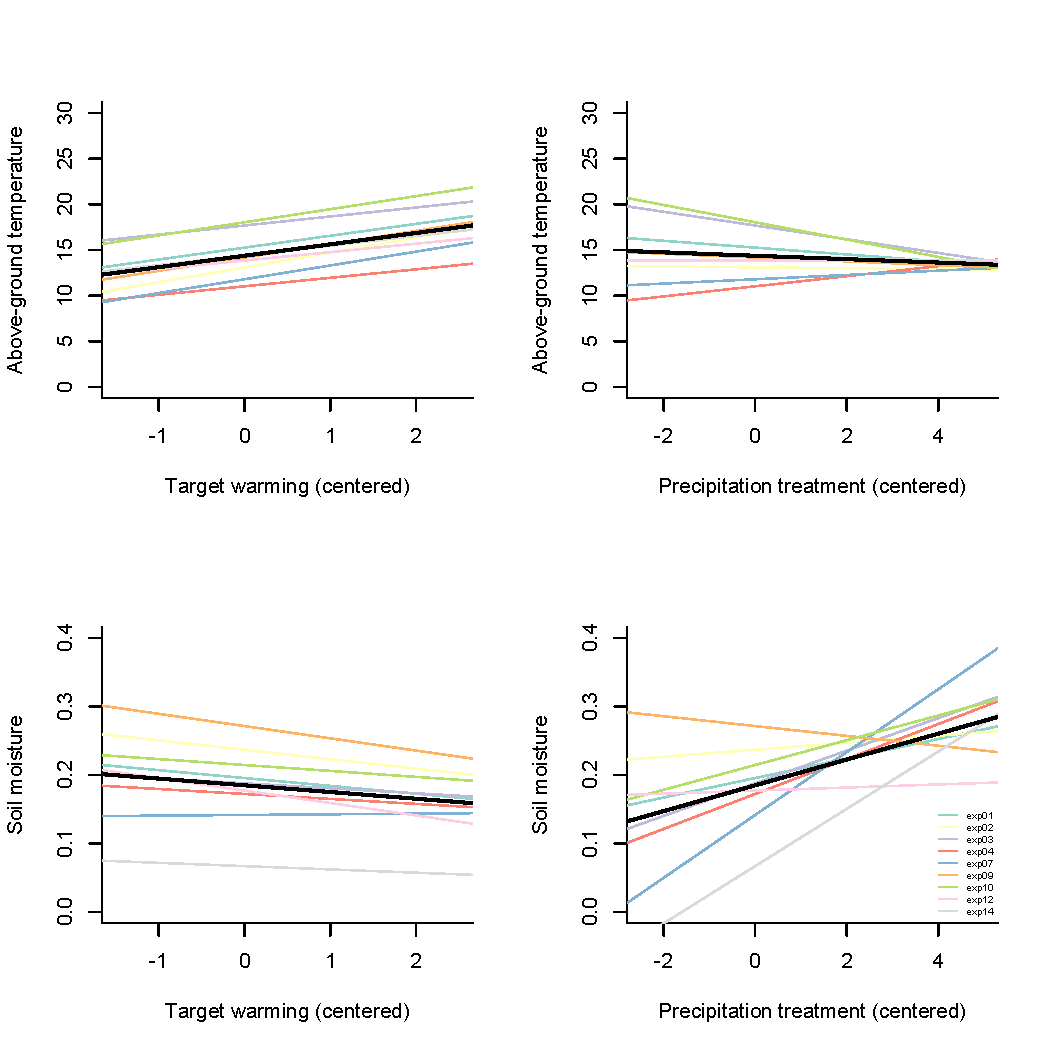
\includegraphics{/Users/aileneettinger/git/radcliffe/Analyses/soilmoisture/figures/smtempvstargtemppreciptreat_lineslmerALL.pdf}
 \caption{\textbf{Effects of target temperature and precipitation treatments on above-ground temperature and soil moisture.}} 
 \label{fig:soilmois}
 \end{figure}

\begin{figure}[h]
\centering
 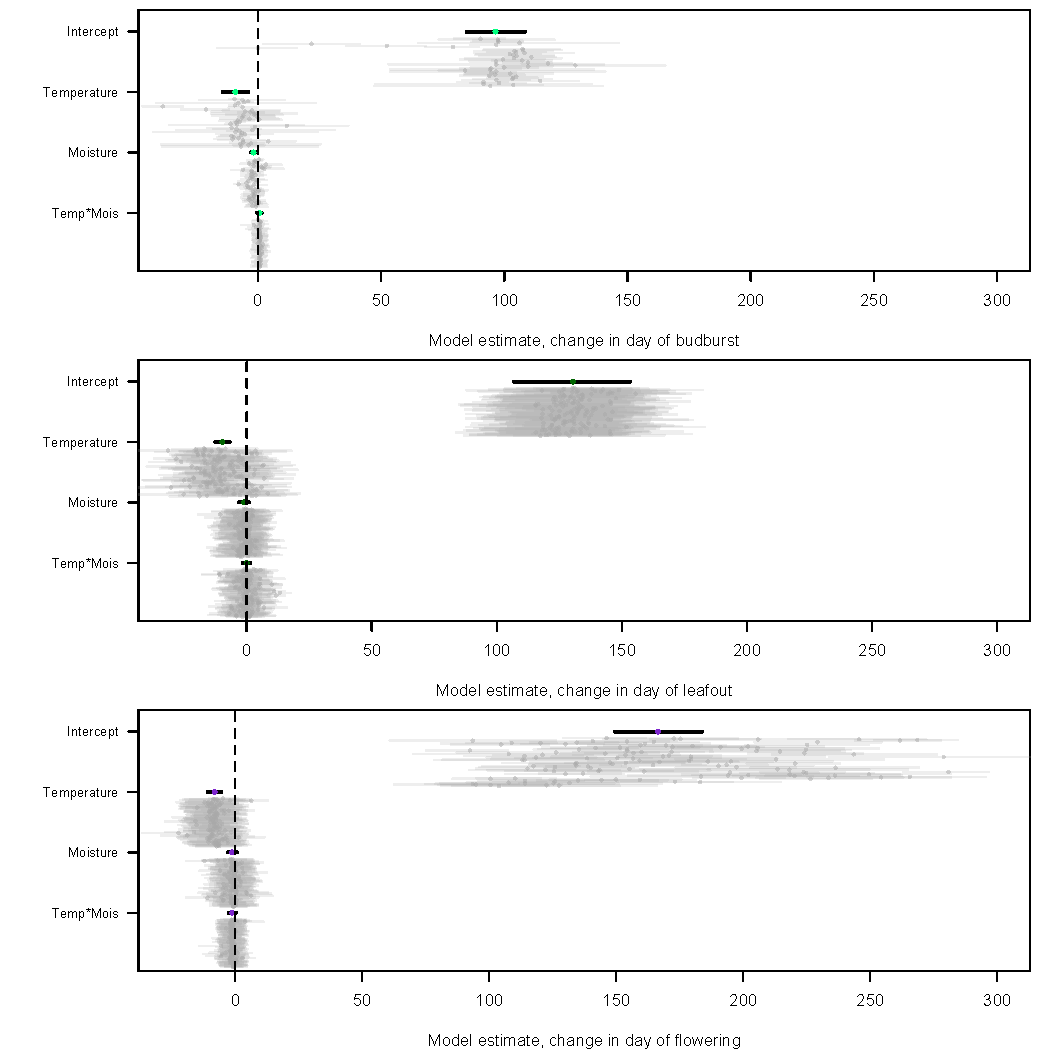
\includegraphics{/Users/aileneettinger/git/radcliffe/Analyses/soilmoisture/figures/m5bbdlodffd.pdf}
 \caption{\textbf{Model coefficients from budburst, leafout, and flowering models (with centered predictors).}} 
 \label{fig:bb}
 \end{figure}

\begin{figure}[h]
\centering
 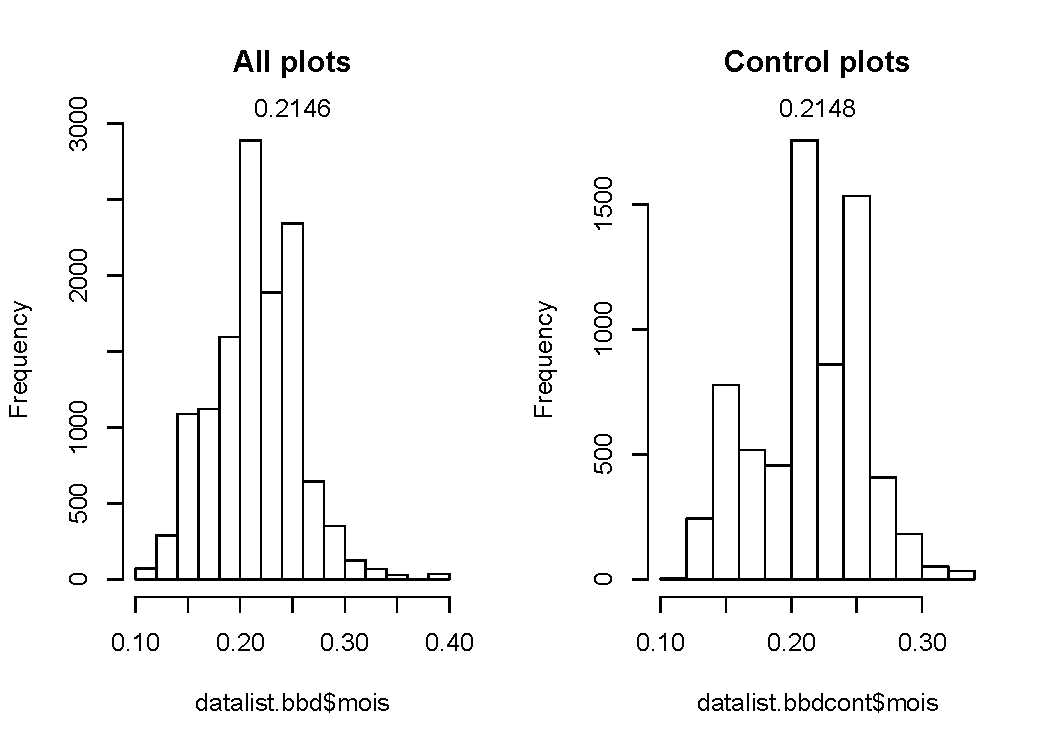
\includegraphics{/Users/aileneettinger/git/radcliffe/Analyses/soilmoisture/figures/soilmoishist_mn.pdf}
 \caption{\textbf{Observed daily soil moisture in all plots verus control plots.}} 
 \label{fig:sm}
 \end{figure}

%begin{figure}[h]
%\centering
% 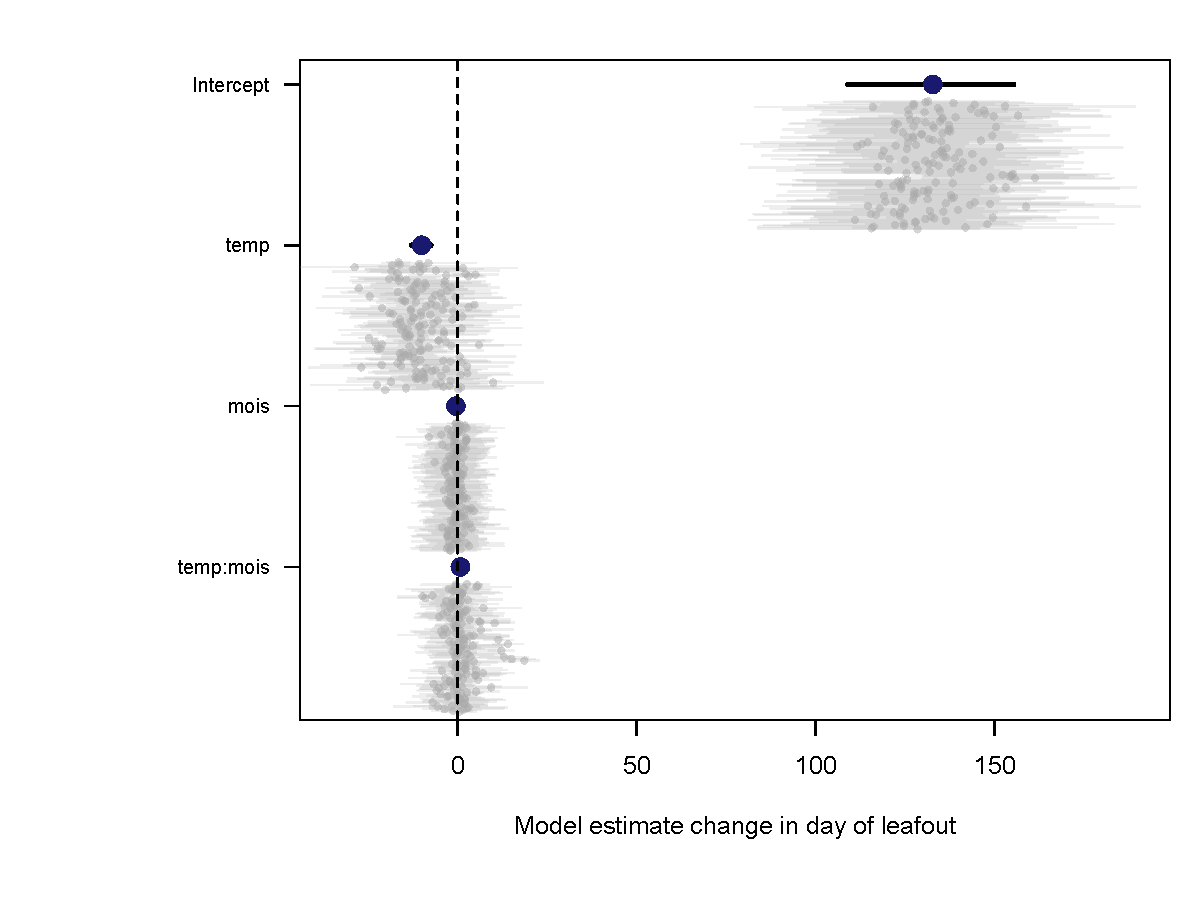
\includegraphics{/Users/aileneettinger/git/radcliffe/Analyses/soilmoisture/figures/m5lod.pdf}
% \caption{\textbf{Model coefficients from leafout model (with centered predictors).}} 
% \label{fig:lo}
% \end{figure}

%\begin{figure}[h]
%\centering
% 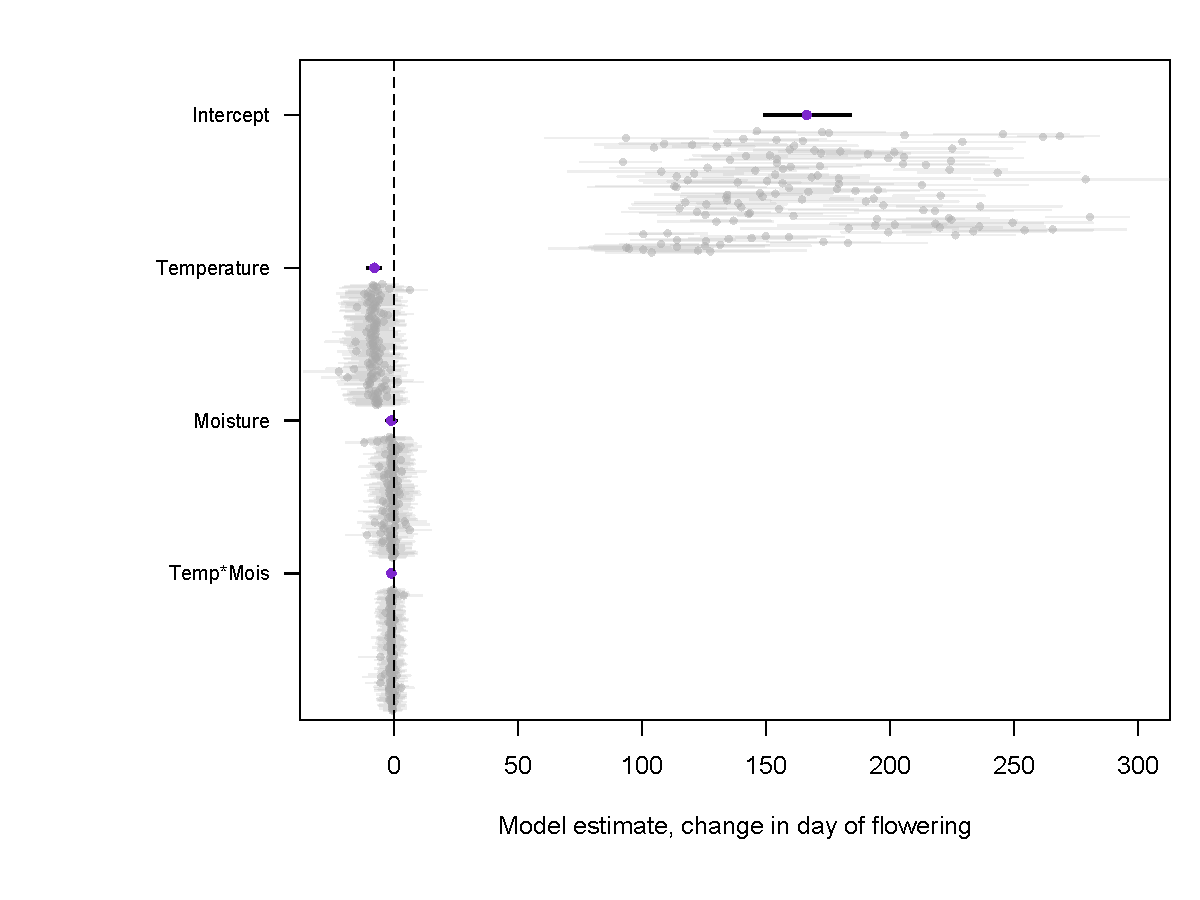
\includegraphics{/Users/aileneettinger/git/radcliffe/Analyses/soilmoisture/figures/m5ffd.pdf}
% \caption{\textbf{Model coefficients from first flower model (with centered predictors).}} 
% \label{fig:ff}
 %\end{figure}
\section* {To do}
\begin{enumerate}
\item Test Yann's theory (that soil moisture affects phenology through its effects on air temperature): fit models with soil temperature instead of air temperature (using same data)- compare coefficients
\item Why is x-axis negative in soil moisture model with centered predictors?
\item Modify Figure 1: color code lines by site, calculate how big effect of precip is and temp is, plot interaction
\item Figure 2: color code dots by species (by BB day of year, from early to late)
\item analyze experimental controls a bit more, before delving into observational comparisons
\end{enumerate}
\section*{References to include}
\begin{enumerate}
\item Later flowering is  associated with low precipitation, at least in part (Crimmins et al 2010)
\end{enumerate}
%%%%%%%%%%%%%%%%%%%%%%%%%%%%%%%%%%%%%%%%
\end{document}
%%%%%%%%%%%%%%%%%%%%%%%%%%%%%%%%%%%%%%%%
